\section{Introduzione alle reti UAV} \label{sec:reti_uav}

% TODO ricontrolla chiarezza e fluidità di tutto il testo
I veicoli aerei senza pilota UAV (Unmanned Aerial Vehicle) sono dei mezzi volanti controllati da remoto, o in alcuni casi, completamente autonomi (Figura \ref{fig:esempi_uav}).
\begin{figure}[t]
    \centering
    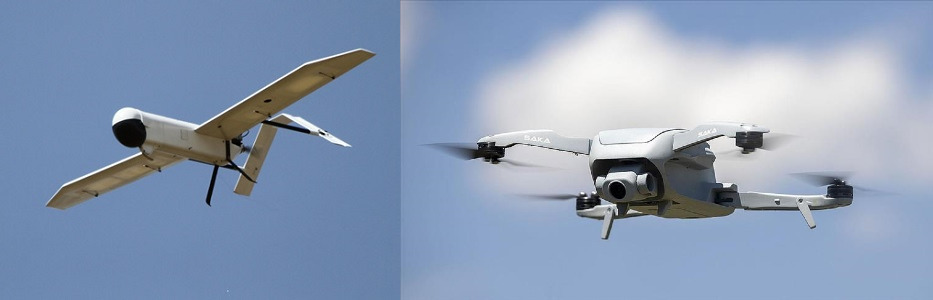
\includegraphics[width=0.8\textwidth]{img/ch1/esempi_uav.jpg}
    \caption{Esempi di dispositivi UAV}
    \label{fig:esempi_uav}
\end{figure}

Le reti UAV \cite{JavaidShumaila2023CaCi} sono dei sistemi multiagente composti da un insieme di \textbf{droni}, eventualmente anche da stazioni a terra (\textbf{Base Stations}, BS), capaci di comunicare tra di loro, che vengono usati come \textbf{nodi di una rete wireless} e svolgono la funzione di \textbf{ripetitori di segnale}; questo sistema è in grado di configurarsi in modo tale da fornire una connessione agli utenti dislocati a terra (Figura \ref{fig:esempio_rete_uav}).

L'adozione di questo paradigma per fornire accesso alla rete presenta diversi vantaggi, ad esempio:
\begin{itemize}

\item regolando l'altitudine dei droni è possibile aggirare agevolmente ostacoli presenti a terra, permettendo di stabilire collegamenti in linea d'area (Line of Sight, LoS)

\item la limitata necessità di strutture fisse a terra permette il dispiegamento dell'infrastruttura di rete in modo rapido, rendendola particolarmente adatta a situazioni di emergenza

\item data l'elevata mobilità dei nodi è possibile riconfigurare facilmente la rete a fronte di variazioni delle necessità da parte degli utenti, ottenendo un'alta flessibilità

\item data la struttura della rete si ha un'alta scalabilità del sistema

\end{itemize}

Un altro aspetto rilevante di questo paradigma è quello che, essendo presente una connessione tra gli agenti, è possibile l'interscambio di informazioni riguardanti l'area circostante di ciascun drone, riuscendo quindi a dare ad ogni singolo agente una visione più completa dell'area attualmente esplorata.

\begin{figure}[t]
    \centering
    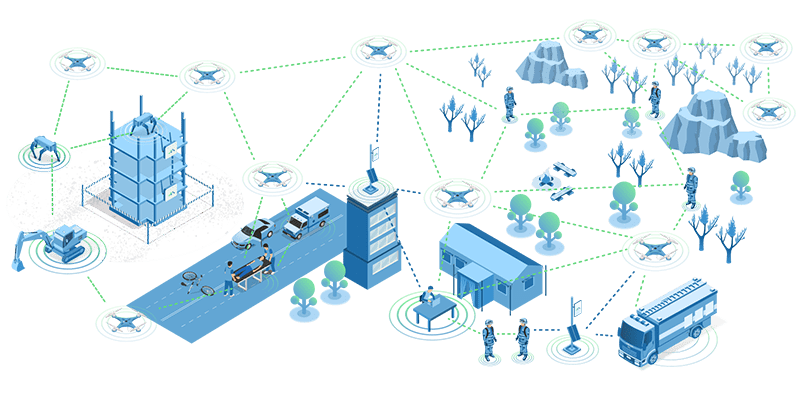
\includegraphics[width=1\textwidth]{img/ch1/uav_network_example.png}
    \caption{Esempio schematico di una rete UAV}
    \label{fig:esempio_rete_uav}
\end{figure}

Nelle reti di telecomunicazioni esistono diversi paradigmi per gestire la comunicazione tra i nodi della rete; uno degli aspetti caratterizzanti di questi paradigmi è la topologia adottata, ovvero la disposizione spaziale dei nodi e dei collegamenti fra di essi.
Per quanto riguarda le reti wireless UAV si possono adottare due tipi di topologie:
\begin{itemize}

\item \textbf{topologia centralizzata}:
ogni nodo deve avere un collegamento diretto con un elemento centrale della rete per essere connesso, ad esempio le BS. Questa tipologia pone in modo evidente un grosso limite all'esplorazione dell'area di interesse, in quanto gli agenti non potranno allontanarsi dai nodi centrali, limitando le zone esplorabili.

\item \textbf{topologia decentralizzata}:
non si identifica un nodo avente maggiore rilevanza, e affinché un nodo sia connesso non importa che abbia un collegamento diretto con un nodo master, ma è sufficiente che vi sia un collegamento indiretto. Questo approccio permette di disporsi in maniera più ampia nella regione da esplorare e di adottare una configurazione maggiormente mutabile nel tempo.
\end{itemize}
\begin{figure}
    \centering
    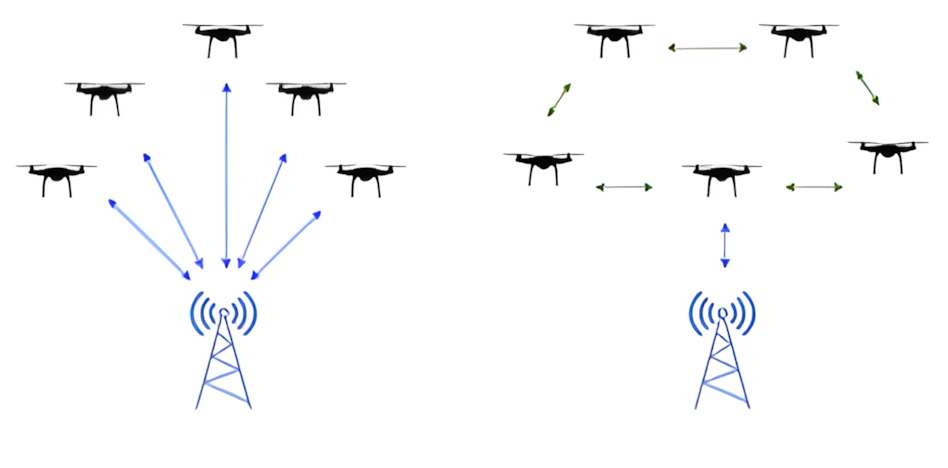
\includegraphics[width=0.8\textwidth]{img/ch1/uav_network_topology.png}
    \caption[Esempi di topologie di rete]{Confronto tra le due topologie di rete: a sinistra vengono mostrati schematicamente dei collegamenti tipici di un network UAV con topologia centralizzata; a destra, lo stesso sistema ma con topologia decentralizzata}
    \label{fig:uav_topology_example}
\end{figure}

Al fine di instaurare una connessione tra agenti può sembrare ragionevole utilizzare la stessa rete utilizzata per la comunicazione con gli utenti. 
Tale approccio tuttavia rischia di limitare l'efficienza complessiva, in quanto la tecnologia utilizzata nelle connessioni tra utenti ed agenti potrebbe non supportare comunicazioni a lunga distanza, riducendo di conseguenza la distribuzione geografica del sistema.
Una strada alternativa per gestire la comunicazione tra UAV può essere quella di utilizzare una rete apposita, detta rete di \textbf{backhaul} \cite{GuanYue2024CUTD}\cite{AlzenadMohamed2016FVBF}; questo comporta una divisione della rete complessiva in due sottoreti, in un certo grado indipendenti tra di loro.
Il vantaggio di utilizzare questa divisione è quello che la rete di backhaul può sfruttare tecnologie di telecomunicazioni a più ampio raggio, come ad esempio la Free Optical Space (FOS) \cite{8938182} o le comunicazioni satellitari \cite{HosseiniNozhan2020UCaC} (Figura \ref{fig:backhaul_example}), in modo che la comunicazione tra agenti non risulti un fattore limitante per la performance del sistema.
\begin{figure}[t]    
    \centering
    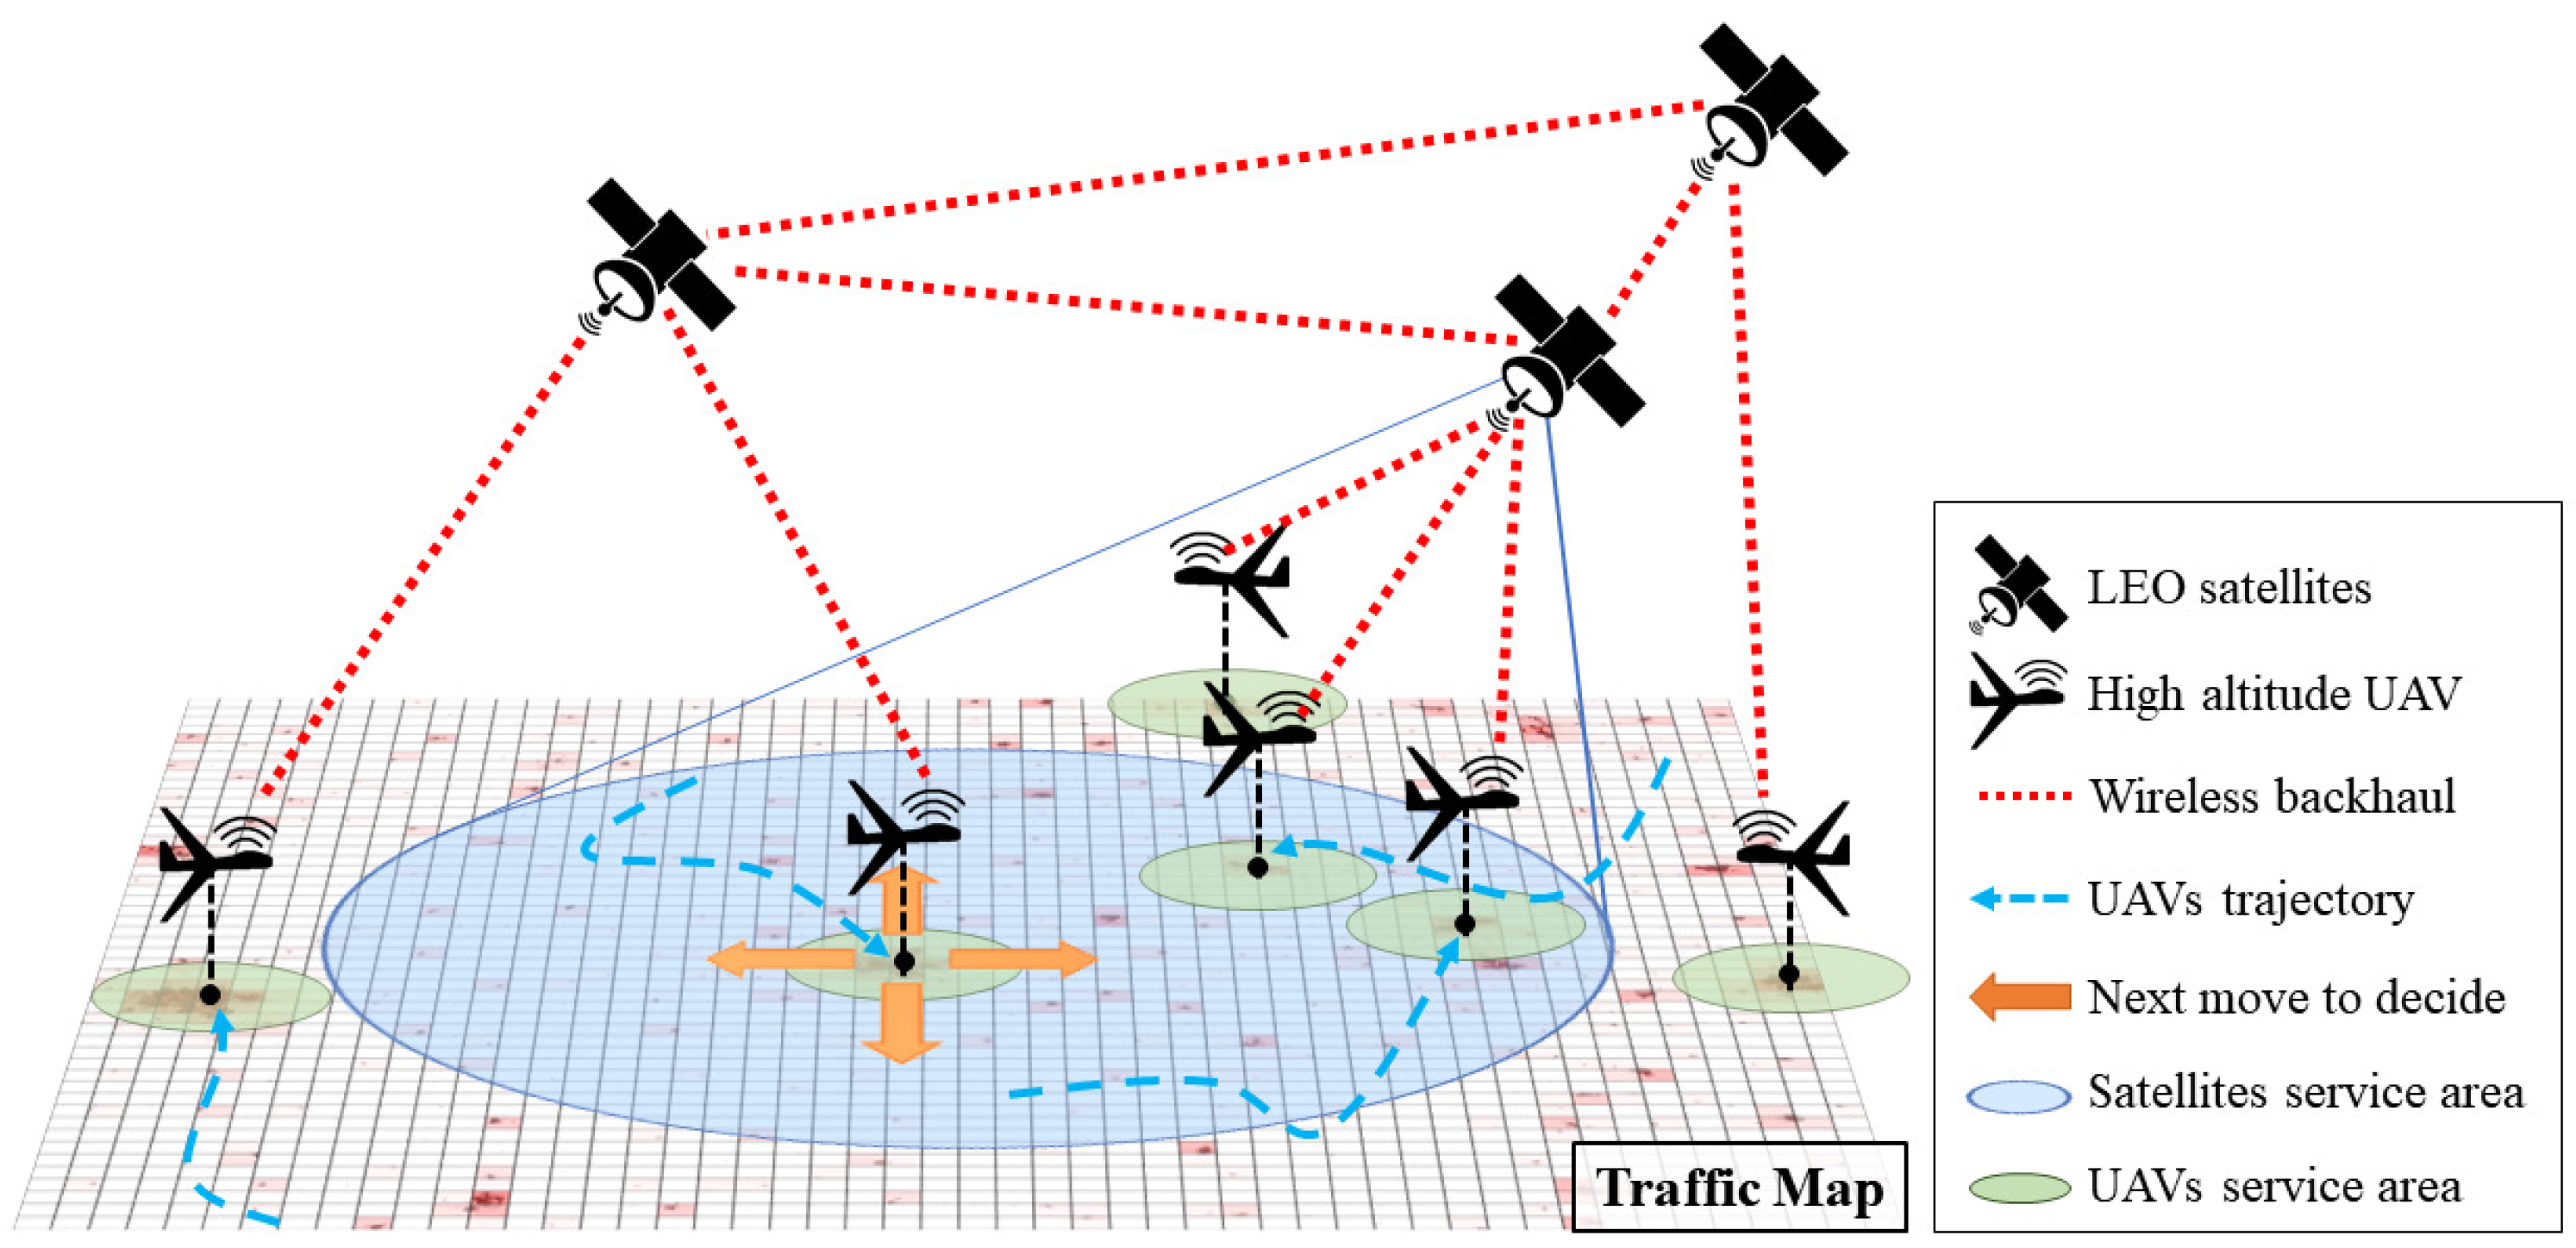
\includegraphics[width=1\textwidth]{img/ch1/satellite_backhaul_network_example.png}
    \caption[Comunicazioni UAV-to-UAV con backhaul satellitare]{Rappresentazione schematica delle comunicazioni UAV-UAV mediante una rete backhaul satellitare.}
    \label{fig:backhaul_example}
\end{figure}